\documentclass[]{article}
\usepackage[left=2.5cm,right=2.5cm,top=2.0cm,bottom=2.5cm]{geometry}
\usepackage{graphicx}
\usepackage{hyperref}
\graphicspath{.}
\title{System Call Proxy Protocol}
\begin{document}
\maketitle

\section{Introduction}

This document describes a distributed dataplane to support clustered
operating system functions. For no strong reason we have selected
triples, or entity-attribte-value(EAV) assertions as the foundation.
Arbitrary length tuples with schema, basically relational tables is another
suitable substrate, as is a simple nested hierarchy. 

We put a little structure around our triples and then address some of the
issues around distributed evaluation of programs that operate on this
EAV graph. 

\section{Triples Model}
Triples came out of the semantic web, in a specification called RDF,
where unfrotuantely the mapping between XML and RDF was left
undefined (\href{https://en.wikipedia.org/wiki/Resource_Description_Framework}).
Objects in the system are given globally unique
identifiers. Each of these objects has a set of properties described
by the attribute field, and each attribute for an entity has exactly
one value. So we can view EAVs as really just a property list or
hashmap.

Since the value can be another entity, triples can also be used to
form a graph of entities with labelled edges. When developing schema
for this system (for some reason we use the word ontology), its quite
common for the attributes themselves to be objects, although this
isn't a usage we will pursue.

The objects of interest in our system are things like:
\begin{itemize}
   \item machines
   \item processes
   \item users
   \item files
\end{itemize}

It shouldn't be contentious that we can use this graph to model
operating system state, in particular the posix-esque semantics of
linux syscalls. If not, hopefully the following details will paint a
better picture.

\subsection{Entities}
Entities are the objects of our system, and to facilitate distribute
evaluation we will also use them as addresses for purposes of
routing. We also need to construct them in such a way that they can
efficiently generated, and that we can never have two objects anywhere
in the world with the same name.

There are probably too many dependencies on the ultimate distribution
methodology to make an authoratative design, but this can serve as
an illustrative example:\\
\vspace{0.2in}
\begin{center}
  \includegraphics[scale=0.8]{entity.pdf}
\end{center}  

\subsection{Attributes}
In many triple setups, the attributes are entities themselves. This allows
attribute metadata such as kind of modifier, historical information, references
into specifications, etc. At the other end of the spectrum attributes are
selected from a small set of predefined integers. For the initial system we propose a middle
ground, that attributes be freeform strings. In order to bring some modicum of
standardization and control to the layout of objects, we introduce a simple
schema definition to publish known keys and support validation. 

\subsection{Values}

\section{Schema}

\section{Commands}

\subsection{set(entity, attribute, value)}
\subsection{get(entity, attribute, value)}
\subsection{copy(dest, source, length)}
\subsection{create(dest, source, length)}

Copies {\em length} bytes from the {\em source} bytestring to the {\em dest}. It
is an error if both the referred objects are not byte strings. For convenience if
the destination is an (entity, attribute) pair which current is unbound, then
the binding is created and set to the bytestring specified by the source address.

As a convenience function, an address which points to an (E, A) that is empty
instantiates the binding with a byte string value of the length. This likely
shouldn't be implicit, but require a distinct command.

\subsection{Addresses}
The {\em source} and {\em dest} parameters are compound addresses. Addresses refer
to byte ranges in values which must be byte strings.

\begin{description}
  \item {value(e, a)}
  \item {offset(A, count)}
\end{description}
Originally addresses were conceived as some kind of nested routing infrastructure, but
that whole line of thought missed the point that entity is does the reachability work
here. There was also a range instead of an offset, but since that implied a length,
that admits a case where the source and destination are mismatched and must throw an
error.

The primary resason that they still live on in the design is the possibility of using
them to express various address translation mechanisms as rewrites as address terms get
evaluated. The most interst example of this would be the translation of a process VMA
to a RDMA window+offset. This along with some RDMA completion plumbing would enable
third party transfers for distributed interleaved requests.


\section{Program Blocks}
Collections of commands are grouped together into {\em blocks}. One reason for doing this
is to avoid alot of request/respose trips when performing compound operations such as
path resolution.

One of the reasons why we defined a command batch was to try to
promote some notion of atomicity or transactionality. Actually
achieving this without substantial investment in the host stack is
likely impossible. In general a systems operation (like writing a
block from a storage device) cant be validated completely in
advance. Nor is it likely that generalized undo strategies for many of
these operations can be developed.

Regardless, there is incremental value in issuing multiple related
updates in a single operation. Batches allow us to bundle multiple
operations to avoid round trips, and thus allow to use a fine-grained
schema which would otherwise be costly. Even if we cant promise a
completely atomic operation, for operations like object contruction we
can validate the entire set of initialization values to ensure that
they are consistent.  Furthermore, we avoid problematic states where
the object is partially initialized.


\subsection{Evaluation}
The block evaluation has semantics designed to make it simple to support multiple
results as streams, at the expensive of having to explain them more carefully.

Take a command in our block, it takes some arguments. In order for these to be chained
and permit other interesting uses, we allow some of these terms to be variables bound at
runtime. So we can express a general copy from A to B where variables are denoted with a '%%' as:
\begin{verbatim}
  get A attr %1
  set B attr %1
\end{verbatim}
  
  We generalize the binding of variables to include multiple values. In logic we would
  say that variables are universally qualified rather than existentially. In programming we
  would say that every command contains an implicit {\tt forall} loop around it. Variables are
  all initialized to to the universe of all values (\textfrac{U} or $\top$).

  At each step in the evalution, constants are treated as unit sets, and for variables
  we take the intersection of the current value with the valid values that that variable
  can take in that expression. This results in a naive implementation of unification. The
  most trivial implmenetation of multiple results is to simply evaluate the succeeding expressions
  for every combination in the intersection.

  So now we can copy all the attribute/value pairs from A to B by allowing {\tt %%1} and {\tt %%2} to
  range over all valid entries.
    
\begin{verbatim}
  get A %1 %2
  set B %1 %2
\end{verbatim}  

For convenience, we define operations on {\tt %%0} to be the union rather than the intersection. Since
a starts out as $\fracmath{U}$, this becomes '\_' or a 'dont care' argument.
  
\subsection{Results/Continuations}
We've painted a picture of an evaluation tree, where we can split work if its worthwhile to do
so, but we haven't discussed how results and errors get propagated back to the original caller. Since we're
not going to really be programming very much of this stuff, lets avoid adding more constructs and just say
that 

  
\subsection{Error handling}




\section{Concurrency}

The current implementation does not provide any global isolation or
serializability for the execution of blocks. If services are provided on top of
a system like Linux, then its very difficult to introduce these concepts because
the underlying facilites aren't 2-phase - they cant in any way promise to commit.

\section{Security}
There is a nice design where blocks are signed by principals, and
contain signed statements of delegated authority. A user might start a
process and sign a statement including the processes new public key
and a set of grants in EAV space.

If we insist that programs can be rewritten by intermediate nodes (for example the interleaved
storage example), then we are opening the door for privledge escalation, because intermediate
nodes must be able to have very permissive grants to handle any clients traffic, and if the
policy of the intermediate and ultimate nodes about the principal differ, then we can easily
violate the policy of the ultimate node.

\end{document}
